%*******************************************
\section{Target Group}
%*******************************************
\label{s:target_group}
This chapter deals with the target group we want to reach with our app.
After defining our target audience we briefly explain how it can be projected to the German population.

\subsection{Target Group definition}
In this section we want to describe the targeted users for our app.
The main condition that must be met is that they can learn something from our app.
That means they are skilled enough to use the app and not too skilled so that they already know everything that the app tells them.
In detail this is modeled by the following conditions.
\begin{description}[leftmargin=0cm]
\item[Attackability] The first precondition is that all our users must meet is that they are possible targets for phishing.
This means they must use the Internet.
They also should use the Internet often enough and have a common trust in the web so that they are in general willing to enter their personal data \cite{divsi2012divsi}.

\item[Android Users] The second precondition is that the users should use an android smartphone.
Our evaluation shows that the app is also usable by iOS users but they are not the target group because they cannot use the app on a regular basis.
\item[Language] The informative parts of our app are texts and they are written in German.
This means the target user should be able to read German texts.
\item[Motivation] The distribution plan for this app is to put it on the Google Play Store and hope that users download and install it.
Therefore, the target user must be willing to learn something about the Internet. According to a study from the DIVSI \cite{divsi2012divsi}, some Internet users are so sure about their knowledge that they are not willing to learn anything else.
We will not be able to reach these users.
\end{description}

\subsection{Projection to Population}
After we have decided what our target group is, we wanted to make sure that we do not exclude too many of the potential users with these preconditions.
In fact, the app can only be useful and successful if a reasonable audience is covered.
To prove this we looked at an extensive survey done by SINUS-Instituts Heidelberg on behalf of Deutschen Instituts f\"{u}r Vertrauen und Sicherheit im Internet (DIVSI) \cite{divsi2012divsi}.
In this survey the authors first looked at 60 persons in detail and found seven types of Internet users that are depicted in \autoref{fig:divsi_milieus}.
Thereafter, they tried to apply the findings to the whole German population by interviewing 2,000 representative persons.
\autoref{fig:divsi_kartoffeln} illustrates the percentage share of the seven Internet types in Germany.
We tried to match our preconditions to these groups. In the following we present our evaluation of each of the groups.

\begin{figure}[hHtbp]
\centering
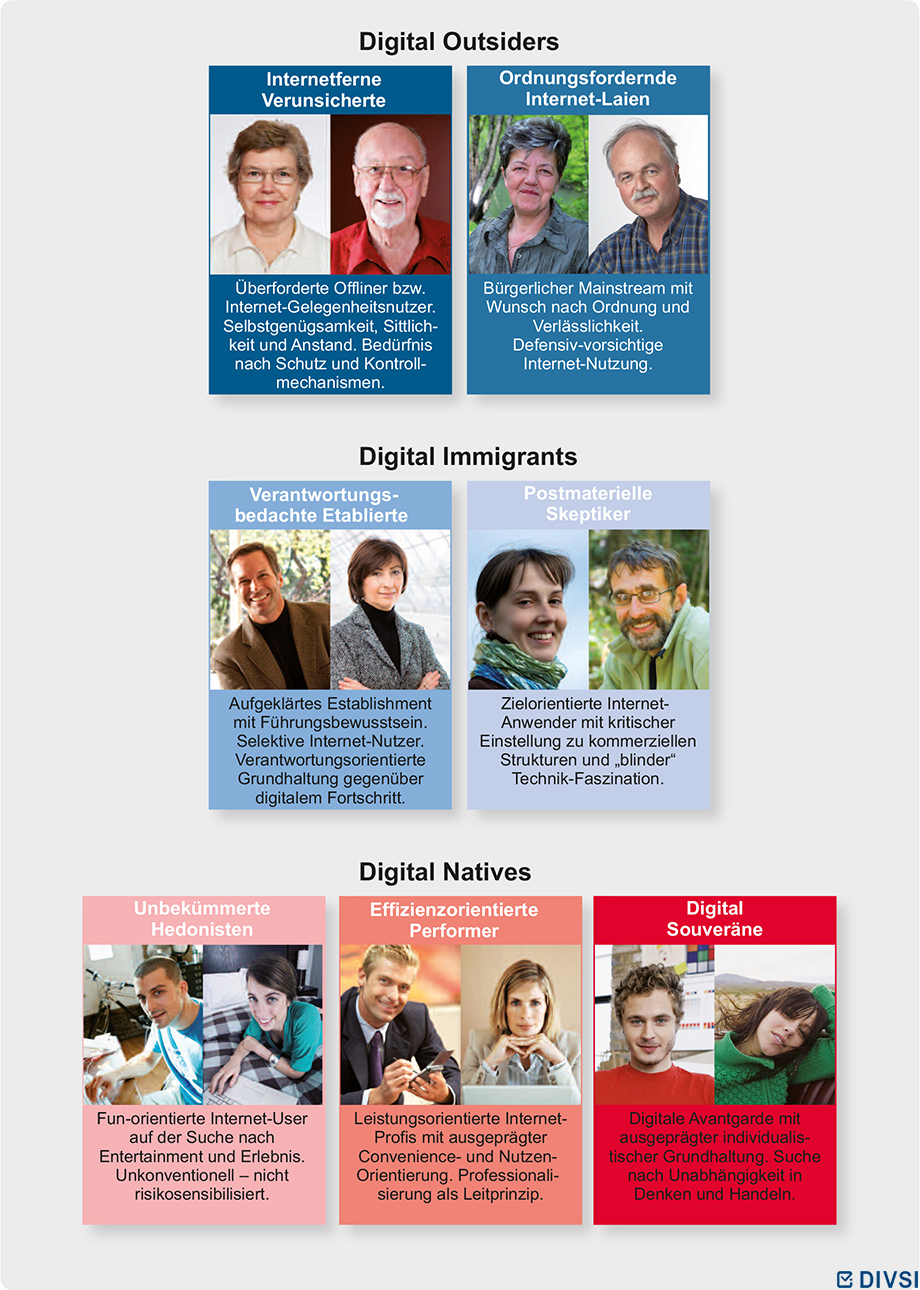
\includegraphics[width=0.9\textwidth]{DIVSI-Milieus.jpg}
\caption{Internet Milleus as defined by DIVSI \cite{divsi2012divsi}}
\label{fig:divsi_milieus}
\end{figure}

\begin{description}[leftmargin=0cm]
\item[Digital Souver\"{a}ne] This group moves naturally on the Internet and is therefore exposed to phishing. They also often use smartphones. We rule them out because they think that they already know the problems of the Internet and hence they would reject a training offer anyways. In fact, this group will likely never download the app.
\item[Effizienzorientierte Performer] This group matches our preconditions because they are using the Internet as well as smartphones. In contrast to the previous group, they are interested in learning something new and see their own learning as an investment in the future. To target this group we should show that you can learn something from this app.
\item[Unbek\"{u}mmerte Hedonisten] This group is also native in the digital worlds but in contrast to the before mentioned groups are not aware of the problems and frauds therein. When they are aware of the problems they seek to secure themselves with automated software instead of concerning themselves with it. Therefore, they are not motivated to use our app.
\item[Postmaterielle Skeptiker] This group is interested in the Internet and uses it frequently. On the other hand they are aware that there are problems and frauds. As they are interested in information on the Internet especially from official sources they might download our app. To target this group we should clearly state that this app is from an university.
\item[Verantwortungsbedachte Etablierte] This group is online regulary and also uses smartphones. They are especially interested in using protection software and actively search information on the Internet. The users of this group do not think that they could protect themselves from the dangers of the Internet and actively seek to change this. Therefore they most likely will appreciate the app. To target this group we should clearly state that this app helps the user to protect himself.
\item[Ordnungsfordernde Internet-Laien] These users are using the Internet rarely. Because of this they are particularly careful when using the Internet and normally do not enter personal data. Therefore, it is not likely that they will use the app. Besides, they usually do not have smartphones.
\item[Internetferne Verunsicherte] These users do not use the Internet. Therefore, they are not exposed to phishing threats.
\end{description}

\begin{figure}[hHtbp]
\centering
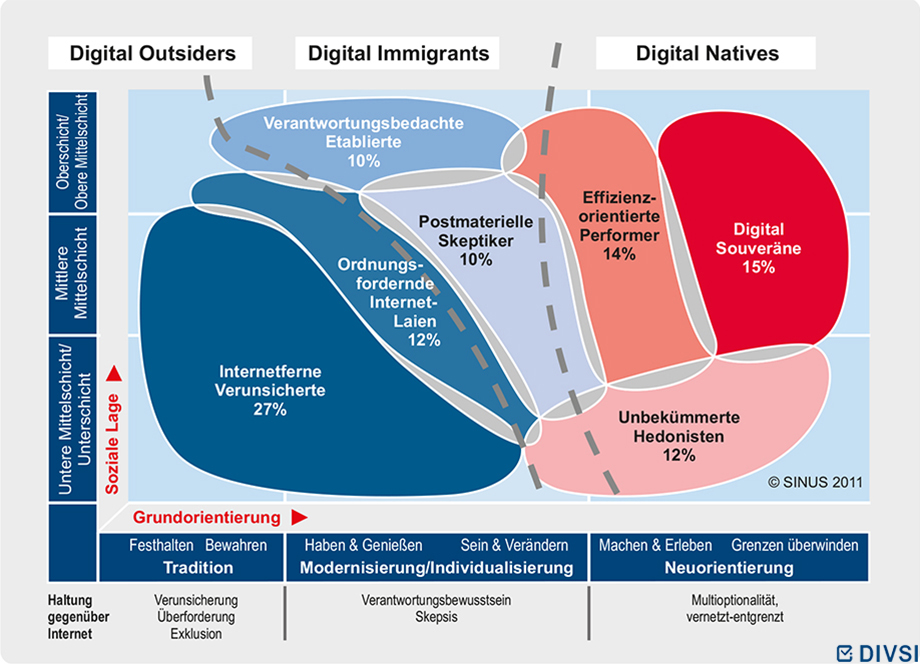
\includegraphics[width=0.56\textwidth]{DIVSI-Kartoffeln.jpg}
\caption{Internet Milleus as defined by DIVSI}
\label{fig:divsi_kartoffeln}
\end{figure}

In conclusion, we consider \textit{Verantwortungsbedachte Etablierte} (10\%),  \textit{Postmaterielle Skeptiker} (10\%),  \textit{Effizienzorientierte Performer} (14\%). In total these are 34\% of the german population.